\section{Experiment}
\label{sec:exp}

\subsection{Experiment Setup}

Our experiments are carried out using DBpedia2014~\cite{dbpedia} and Probase~\cite{wu2012probase}. We draw entities and their relationships from DBpedia, and the concept infomation from Probase.

\subsection{Results}

We show some of the relations that has been retrieved by our method in Table~\ref{tab:results}.
The first 2 columns show the query entity pair.
The 3rd column is the relation retrieved by ERF with a confidence score in the 4th column.
Note that we combine the relation of $\langle e_1,e_2\rangle$ and $\langle e2,e1\rangle$ into one single result.
For example the relation \at{commander} of \at{<adolf hitler,world war ii>} is actually that of \at{<world war ii, adolf hilter>}
% Table generated by Excel2LaTeX from sheet 'Sheet1'
\begin{table}[ht!]
  \centering
  \caption{First three results produced by ERF}
    \begin{tabular}{cccr}
    \toprule
    Entity1 & Entity2 & Relation & Score \\
    \midrule
    \multicolumn{1}{c}{\multirow{3}{*}{\parbox{1cm}{ Sherlock Holmes}}} & \multicolumn{1}{c}{\multirow{3}[0]{*}{united kingdom}} & anthem & 0.007079 \\
    \multicolumn{1}{c}{} & \multicolumn{1}{c}{} & firstAppearance & 0.004487 \\
    \multicolumn{1}{c}{} & \multicolumn{1}{c}{} & allegiance & 0.004357 \\
    \hline
    \multicolumn{1}{c}{\multirow{3}{*}{\parbox{1cm}{\centering apple}}} & \multicolumn{1}{c}{\multirow{3}[0]{*}{steve jobs}} & foundedBy & 0.015439 \\
    \multicolumn{1}{c}{} & \multicolumn{1}{c}{} & keyPerson & 0.009932 \\
    \multicolumn{1}{c}{} & \multicolumn{1}{c}{} & successor & 0.008069 \\
    \hline
    \multicolumn{1}{c}{\multirow{3}{*}{\parbox{1cm}{\centering Adolf Hitler}}} & \multicolumn{1}{c}{\multirow{3}[0]{*}{world war ii}} & commander & 0.037712 \\
    \multicolumn{1}{c}{} & \multicolumn{1}{c}{} & battle & 0.022161 \\
    \multicolumn{1}{c}{} & \multicolumn{1}{c}{} & ceo   & 2.44E-05 \\
    \hline
    \multicolumn{1}{c}{\multirow{3}{*}{\parbox{1cm}{\centering Microsoft}}} & \multicolumn{1}{c}{\multirow{3}[0]{*}{redmond}} & locationCity & 0.082507 \\
    \multicolumn{1}{c}{} & \multicolumn{1}{c}{} & foundationPlace & 0.047192 \\
    \multicolumn{1}{c}{} & \multicolumn{1}{c}{} & location & 0.036916 \\
    \hline
    \multicolumn{1}{c}{\multirow{3}{*}{Titanic}} & \multicolumn{1}{c}{\multirow{3}[0]{*}{James Cameron}} & director & 0.124407 \\
    \multicolumn{1}{c}{} & \multicolumn{1}{c}{} & cinematography & 0.096447 \\
    \multicolumn{1}{c}{} & \multicolumn{1}{c}{} & editing & 0.080134 \\
    \hline
    \multicolumn{1}{c}{\multirow{3}{*}{Titanic}} & \multicolumn{1}{c}{\multirow{3}[0]{*}{Leonardo Dicaprio}} & starring & 0.049689 \\
    \multicolumn{1}{c}{} & \multicolumn{1}{c}{} & narrator & 0.037267 \\
    \multicolumn{1}{c}{} & \multicolumn{1}{c}{} & producer & 0.01306 \\
    \hline
    \multicolumn{1}{c}{\multirow{3}{*}{\parbox{1cm}{\centering Harry Potter}}} & \multicolumn{1}{c}{\multirow{3}[0]{*}{J K rowling}} & notableWork & 0.016965 \\
    \multicolumn{1}{c}{} & \multicolumn{1}{c}{} & author & 0.015514 \\
    \multicolumn{1}{c}{} & \multicolumn{1}{c}{} & coverArtist & 0.014906 \\
    \bottomrule
    \end{tabular}%
  \label{tab:results}%
\end{table}%


\subsection{Evaluation}
In this subsection we evaluate our ERF system by several means.
Given 2 entities, our system produce the most plausible topK relation between the 2 entities.
Hence we use $nDCG@K$ and $Precision@K$ to as our evaluation metric.

The result is shown in Table~\ref{tab:ndcg}.

\begin{table}[htbp]
  \centering
  \caption{Evaluation Result}
    \begin{tabular}{rr}
    \toprule
    mesure & value \\
    \midrule
    nDCG@3 & 0.945 \\
    nDCG@5 & 0.941 \\
    precision@3 & 0.88 \\
    precision@5 & 0.76 \\
    MAP@3 & 0.902 \\
    MAP@5 & 0.907 \\

    \bottomrule
    \end{tabular}%
  \label{tab:ndcg}%
\end{table}%


We use the direct retrieval as a baseline.
We randomly select 50 paragraph, and take only the abstract part.
We consider the linked entities as the right part of the relation explanation input and source entity as the left part.
Compared with baseline, i.e. DBpedia original(we assume 0 if the entity has no relation can be retrieved from database and otherwise 1), our ERF method improves the precision by 15.77%.
The result is reported in Table~\ref{tab:precision_compare}

\begin{table}[htbp]
  \centering
  \caption{Precision@1 Compared With Baseline}
    \begin{tabular}{rrr}
    \toprule
         & P@1  & \%Improv. \\
    \midrule
    Dbpedia direct & 0.64 & -- \\
    ERF  & 0.83 & 15.77 \\
    \bottomrule
    \end{tabular}%
  \label{tab:precision_compare}%
\end{table}%



\subsection{Head Concept Vs Original Concept}

To further justify the effectiveness of our recalculation of probability, we present the contrast result in Table.~\ref{tab:rerank}.



\begin{table*}[htbp!]
  \centering
  \caption{Rerank comparation}
    \begin{tabular}{llrrlrr}
    \toprule
    \multicolumn{1}{c}{} & \multicolumn{3}{c}{aggregated} & \multicolumn{3}{c}{original head concepts} \\
    \midrule
    \multicolumn{1}{c}{Entity} & agg head & agg count & agg prob & org head & org count & org prob \\
    \midrule
    \multicolumn{1}{c}{\multirow{10}[0]{*}{shanghai}} & city  & 1311  & 0.829222 & city  & 644   & 0.407337 \\
    \multicolumn{1}{c}{} & region & 46    & 0.029096 & region & 27    & 0.017078 \\
    \multicolumn{1}{c}{} & area  & 42    & 0.026565 & metropolis & 23    & 0.014548 \\
    \multicolumn{1}{c}{} & metropolis & 26    & 0.016445 & megacities & 15    & 0.009488 \\
    \multicolumn{1}{c}{} & port  & 20    & 0.01265 & market & 15    & 0.009488 \\
    \multicolumn{1}{c}{} & market & 19    & 0.012018 & location & 15    & 0.009488 \\
    \multicolumn{1}{c}{} & centre & 18    & 0.011385 & port  & 9     & 0.005693 \\
    \multicolumn{1}{c}{} & location & 17    & 0.010753 & locality & 6     & 0.003795 \\
    \multicolumn{1}{c}{} & megacities & 15    & 0.009488 & locale & 5     & 0.003163 \\
    \multicolumn{1}{c}{} & center & 11    & 0.006958 & seaport & 4     & 0.00253 \\
          &       &       &       &       &       &  \\
    \multicolumn{1}{c}{\multirow{10}[0]{*}{bill gates}} & leader & 46    & 0.140244 & billionaire & 37    & 0.112805 \\
    \multicolumn{1}{c}{} & billionaire & 44    & 0.134146 & entrepreneur & 28    & 0.085366 \\
    \multicolumn{1}{c}{} & entrepreneur & 41    & 0.125 & philanthropist & 23    & 0.070122 \\
    \multicolumn{1}{c}{} & philanthropist & 30    & 0.091463 & celebrity & 15    & 0.045732 \\
    \multicolumn{1}{c}{} & celebrity & 20    & 0.060976 & leader & 9     & 0.027439 \\
    \multicolumn{1}{c}{} & person & 16    & 0.04878 & innovator & 6     & 0.018293 \\
    \multicolumn{1}{c}{} & figure & 11    & 0.033537 & personality & 5     & 0.015244 \\
    \multicolumn{1}{c}{} & innovator & 8     & 0.02439 & expert & 5     & 0.015244 \\
    \multicolumn{1}{c}{} & luminary & 8     & 0.02439 & folks & 4     & 0.012195 \\
    \multicolumn{1}{c}{} & individual & 7     & 0.021341 & icon  & 4     & 0.012195 \\
          &       &       &       &       &       &  \\
    \multicolumn{1}{c}{\multirow{10}[0]{*}{samsung}} & company & 1030  & 0.376875 & company & 816   & 0.298573 \\
    \multicolumn{1}{c}{} & brand & 829   & 0.30333 & brand & 561   & 0.205269 \\
    \multicolumn{1}{c}{} & manufacturer & 238   & 0.087084 & client & 42    & 0.015368 \\
    \multicolumn{1}{c}{} & maker & 112   & 0.040981 & firm  & 39    & 0.01427 \\
    \multicolumn{1}{c}{} & player & 60    & 0.021954 & rival & 38    & 0.013904 \\
    \multicolumn{1}{c}{} & phone & 60    & 0.021954 & player & 33    & 0.012075 \\
    \multicolumn{1}{c}{} & giant & 51    & 0.018661 & phone & 30    & 0.010977 \\
    \multicolumn{1}{c}{} & firm  & 49    & 0.017929 & conglomerate & 19    & 0.006952 \\
    \multicolumn{1}{c}{} & name  & 49    & 0.017929 & corporation & 19    & 0.006952 \\
    \multicolumn{1}{c}{} & conglomerate & 42    & 0.015368 & partner & 12    & 0.004391 \\
          &       &       &       &       &       &  \\
    \multicolumn{1}{c}{\multirow{10}[0]{*}{mona lisa}} & painting & 56    & 0.4   & painting & 33    & 0.235714 \\
    \multicolumn{1}{c}{} & masterpiece & 21    & 0.15  & masterpiece & 16    & 0.114286 \\
    \multicolumn{1}{c}{} & work  & 20    & 0.142857 & work  & 10    & 0.071429 \\
    \multicolumn{1}{c}{} & film  & 6     & 0.042857 & film  & 5     & 0.035714 \\
    \multicolumn{1}{c}{} & image & 5     & 0.035714 & image & 3     & 0.021429 \\
    \multicolumn{1}{c}{} & artwork & 4     & 0.028571 & picture & 3     & 0.021429 \\
    \multicolumn{1}{c}{} & portrait & 4     & 0.028571 & treasure & 2     & 0.014286 \\
    \multicolumn{1}{c}{} & piece & 4     & 0.028571 & song  & 2     & 0.014286 \\
    \multicolumn{1}{c}{} & picture & 3     & 0.021429 & icon  & 2     & 0.014286 \\
    \multicolumn{1}{c}{} & figure & 3     & 0.021429 & artwork & 1     & 0.007143 \\
    \bottomrule

    \end{tabular}%
  \label{tab:rerank}%
\end{table*}%



%\subsection{Find alias}

%\subsubsection{compare}
%
%In this section we compare $ P(<c_1,c_2 >|a )$ with $ P(c_1|a) \times P(c_2|a)$ to show that

\subsection{Effectiveness of alpha}



\subsection{Sense Disambiguation}

We can solve the problem of sense disambiguation problem well by applying this method since there are many entities belongs to the same concept and we only consider topK $(c_1,c_2)$ pairs that has high typicality $P( (c_1,c_2) |a)$, so that the weird $(c_1,c_2)$ patterns as manifest in Example.~\ref{exa:sd} can be easily filtered.

\begin{figure}[!htb]
\centering 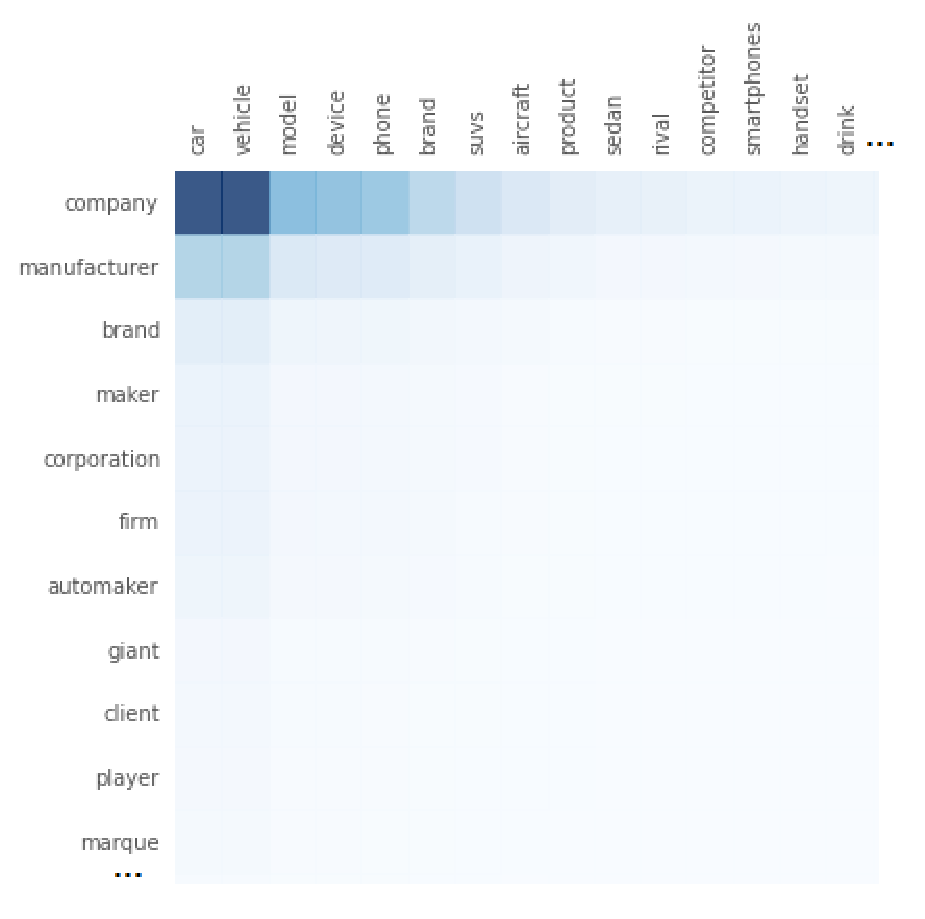
\epsfig{file=resources/ev_plot_manufacturer.eps,width=2.5in}
\caption{$(c_1,c_2$) plot for attribute \term{Manufacturer}} \label{fig:evplot}
\end{figure}

\begin{example}[Sense Disambiguation]
Consider the following $(e1,a,e2)$ tuple \term{(iphone, manufacturer, apple)}. Suppose it is our query, where \term{apple}'s sense can either be a kind of \term{fruit} or a \term{company}.
Fig.~\ref{fig:evplot} is a heatmap for all the concepts pairs $(c_1,c_2)$ of attributes \term{manufacturer}. The horizontal axis represents the $e_1$ and the vertical axis stands for $e_2$. The darker the blue is, the higher typicality it will be. In Fig.~\ref{fig:evplot}, We can observe that the top concepts of $e_2$ in the heatmap are \term{company, manufacturer,...} and top 10 pairs also does not include \term{fruit}. The intuition for this is that there exists thousands of $(e1,a,e2)$ tuple such as \term{(BMW\_Z4,manufacturer,BMW),(PlayStation\_4,manufacturer,Sony)} other than \term{(iphone, manufacturer, apple)} tuple, which results in a reasonable distribution.
\label{exa:sd}
\end{example}



%\subsection{Selectional Preference}
